% O propósito da seção de resultados, como o próprio nome indica, é revelar o que foi encontrado na pesquisa. Essa parte do artigo estará composta dos dados relevantes obtidos e sintetizados pelo autor. 

% Nesta seção, você deverá apresentar todos os elementos solicitados no mapa mental relacionados ao seu projeto: diagramas, protótipos, modelo de negócios, principais funções e componentes desenvolvidos. Para tanto, na subseção a seguir, você poderá consultar como é feita a inserção de figuras, fluxogramas, fotografias, gráficos, tabelas e quadros.


\subsection*{Kanban}

O monitoramento pelo logbook do GitHub, torna a organização do projeto ainda mais eficaz. O GitHub permite um acompanhamento detalhado de cada etapa, com transparência total nas tarefas e progresso da equipe. O logbook facilita o registro de cada atividade. Isso resulta em uma gestão de projeto ágil, organizada e colaborativa, garantindo a entrega de valor em ciclos curtos e controlados. A seguir três fases do kanban durante uma semana: Na \Cref{fig:1}, há quatro tarefas para começar; já na \Cref{fig:2}, a tarefa "Banner" está em progresso; na \Cref{fig:3} já não há mais tarefas para serem iniciadas, todas foram finalizadas apenas "LaTex - artigo" esta em progresso.

\begin{figure}[H]
    \centering
    \caption{1º visão}%
    \label{fig:1}
    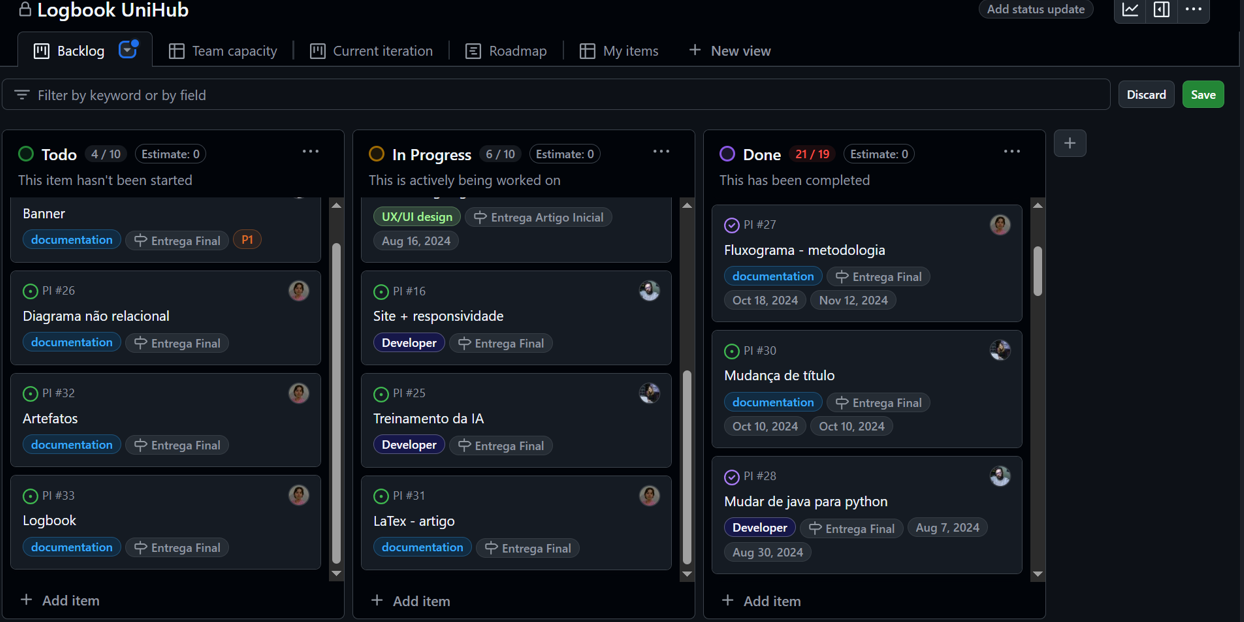
\includegraphics[scale=.38]{kan1}
    \SourceOrNote{Autoria Própria (2024)}
    \end{figure}


    \begin{figure}[H]
        \centering
        \caption{2º visão}%
        \label{fig:2}
        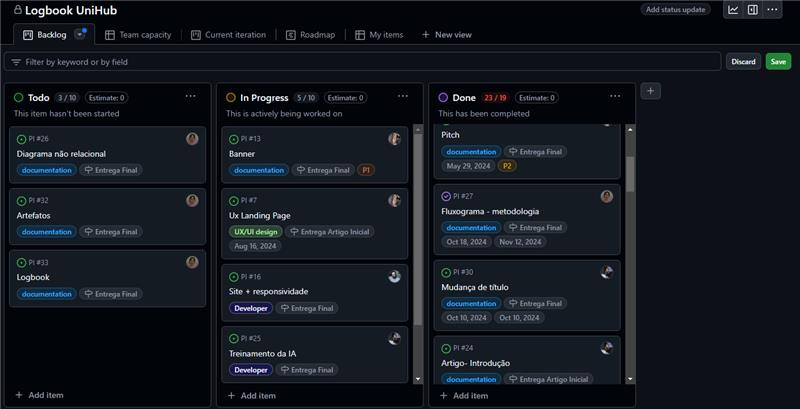
\includegraphics[scale=.6]{kan2}
        \SourceOrNote{Autoria Própria (2024)}
        \end{figure}


        \begin{figure}[H]
            \centering
            \caption{3º visão}%
            \label{fig:3}
            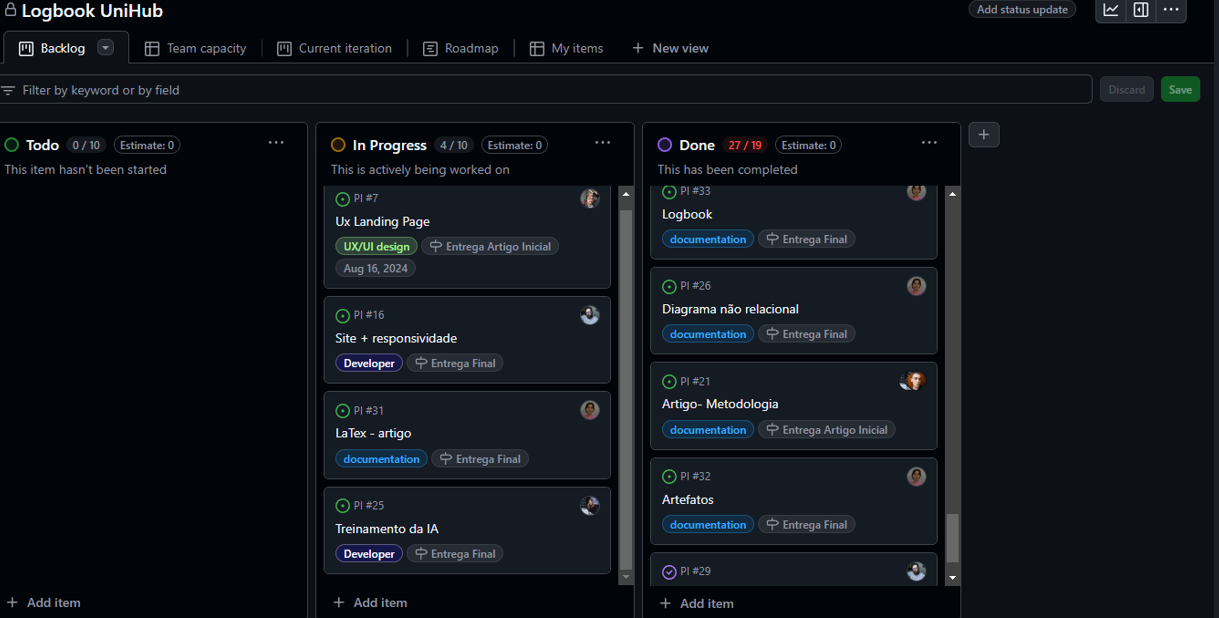
\includegraphics[scale=.38]{kan3}
            \SourceOrNote{Autoria Própria (2024)}
            \end{figure}
            


\subsection*{Diagrama de Banco de Dados Não Relacional}

O diagrama foi pensando na seguinte forma, a tabela indexações registra os dados relacionados ao conteúdo do site em si, como local de armazenamento, url da página, se será liberada ou bloqueada, e o termo que justifica este possível bloqueio. Além das informações de data e máquina que ocasionou essa indexação, por acessá-la.
Já a tabela acessos, registra os dados dos demais acessos a um site já verificado e indexado, por isso apenas possui. Esta tabela serve para fins estatísticos, portanto, apresenta a url da página, data, hora e ip da máquina por onde foi acessado.
A tabela funcionarios registra os dados relacionados aos colaboradores de uma instituição. Cada documento armazena informações pessoais, como nome, e-mail, telefone e uma URL para foto de perfil do usuário. Além disso, inclui o campo instituicao, que é um documento aninhado, em qual são armazenados os dados de outras instituições que o usuário possa estar vinculado, como o nome, CNPJ e o \textit{endpoint} da \textit{Application Programming Interface} (API) utilizado para integrações ou consultas relacionadas à instituição. Também são registradas as permissões atribuídas a cada funcionário, detalhando os tipos de ações que podem ser realizadas no sistema, como criar, editar ou deletar informações.

\begin{figure}[H]
    \centering
    \caption{Diagrama de Banco de Dados NoSQL}%
    \label{fig:banco}
    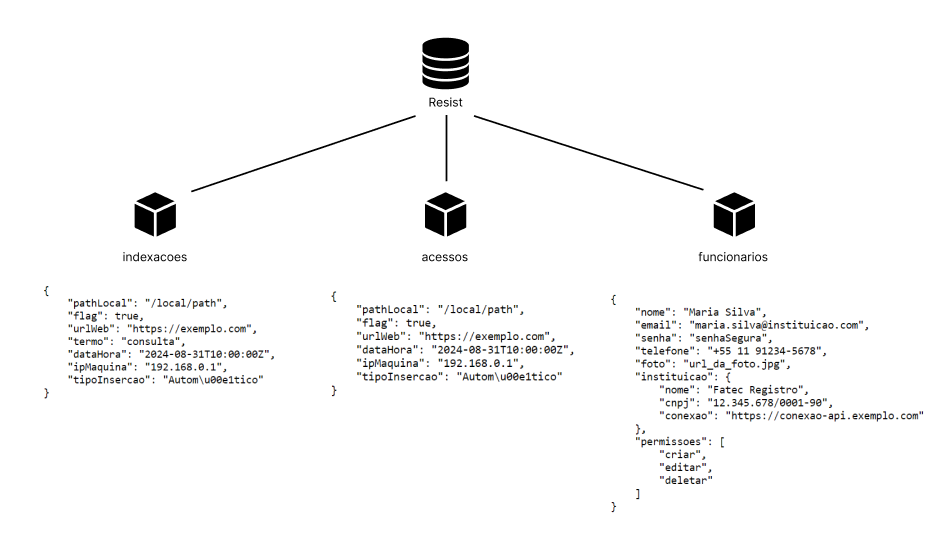
\includegraphics[scale=.6]{banco}
    \SourceOrNote{Autoria Própria (2024)}
    \end{figure}

\subsection*{Aplicação Desktop}

O desenvolvimento da aplicação Desktop foi realizada utilizando a linguagem de programação Python, este sistema desempenha o papel de extrair o conteúdo dos sites, para que possam ser analisados em busca de possíveis contextos injuriosos, e caso seja encontrado, bloqueá-los na rede local.

Utilizando o \textit{Requests}\footnote{biblioteca capaz de extrair o conteúdo textual de websites}, obteve-se um sistema capaz de monitorar os acessos relatados pelo Squid. A aplicação retorna para cada acesso registrado a Url, data, hora e ip da máquina que solicitou o acesso. Neste ponto, a aplicação confere se o site já foi verificado antes, e em caso negativo, realiza todo o processo de extração e verificação do teor da página.

No entanto, a aplicação ainda não é capaz de verificar contextos, pois ainda não houve a integração com a Inteligência Artificial, por limitações com o hardware usado no treinamento, o que limita a detecção do sistema. Portanto, o programa realiza uma leitura da página em busca de uma palavra específica, e a presença ou ausência desta palavra será o fator determinante para bloqueio ou permissão do acesso a esta página, caso determinado site seja bloqueado uma notificação é enviada ao usuário (Figura x) e a página não poderá ser vista pelo usuário (Figura Y). 

A Url da página é armazenada em um banco de dados, para que seja possível visualizar se a página está liberada ou não, e qual palavra ou frase motivou seu bloqueio.
Após a verificação, o sistema também utiliza os dados recuperados para registrar no banco cada acesso, o que permitirá a geração de dados detalhados, que serão utilizados para criar gráficos e relatórios acessíveis via Web para os gestores das instituições.

\subsection*{Website para Gestores}

O Website será principalmente utilizado pelos administradores e gestores de escolas, para visualizar os gráficos e relatórios citados anteriormente. Exibindo estes dados e registros de forma dinâmica, o sistema torna-se uma ferramenta para que os mesmos possam identificar as salas ou setores onde pesquisas de teor discriminatório estão ocorrendo com mais frequência, além da incidência e médias de bloqueio em cada área, entre outros.

\begin{figure}[H]
    \centering
    \caption{Dashboard}%
    \label{fig:dashboard}
    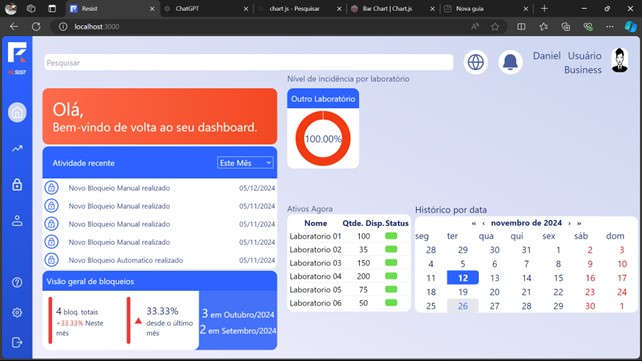
\includegraphics[scale=.7]{dashboard1}
    \SourceOrNote{Autoria Própria (2024)}
    \end{figure}

    
    A \Cref{fig:dashboard} ilustra a tela inicial, tratando-se de um \textit{Dashboard} que proporciona um resumo das informações coletadas, como a atividade recente, que apresenta todas as atualizações do ambiente; visão geral dos bloqueios, trazendo a quantidade de bloqueios e a evolução em relação ao mês anterior; nível de incidência por laboratório (no exemplo, tratam-se de laboratórios de informática em um ambiente escolar); histórico por data, e os laboratórios que estão ativos no momento.


    \begin{figure}[H]
        \centering
        \caption{Estatísticas}%
        \label{fig:estatisticas}
        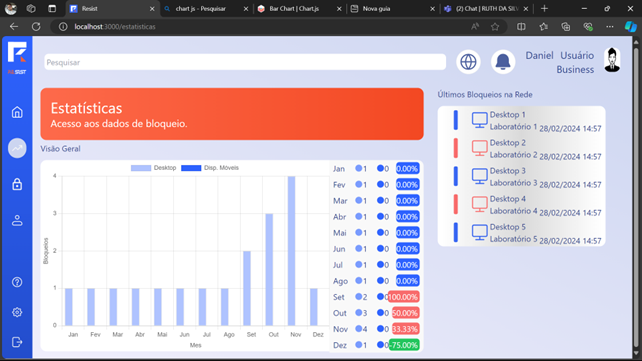
\includegraphics[scale=.7]{estatisticas2}
        \SourceOrNote{Autoria Própria (2024)}
        \end{figure}
        
        A \Cref{fig:estatisticas} exibe a aba de estatísticas, onde há uma visualização aprofundada dos dados de bloqueio, exibindo a quantidade de bloqueios em dispositivos móveis e \textit{Desktop}, uma comparação do aumento ou diminuição mês-a-mês, e alguns dos últimos bloqueios na rede.
        
     \begin{figure}[H]
        \centering
        \caption{Bloqueios}%
        \label{fig:bloqueios}
        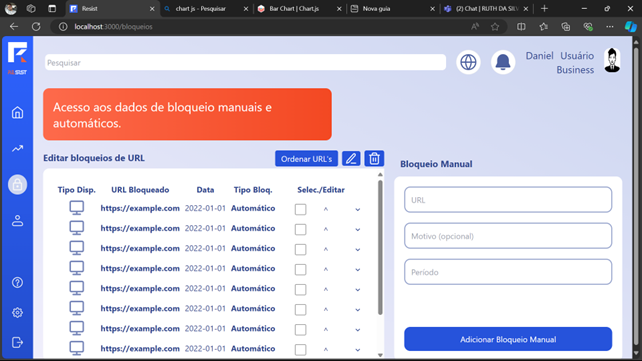
\includegraphics[scale=.7]{bloqueios3}
        \SourceOrNote{Autoria Própria (2024)}
        \end{figure}

    A página bloqueios, representada na \Cref{fig:bloqueios}, exibe uma visão aprofundada sobre cada bloqueio realizado. É exibida uma tabela com a URL bloqueada, a data do bloqueio e se foi manual ou automático. A página disponibiliza ainda uma funcionalidade para bloquear um Website manualmente, especificando o motivo e período do bloqueio. É possível editar os bloqueios já realizados, para caso seja necessário cancelá-los.

    \begin{figure}[H]
        \centering
        \caption{Notificação}%
        \label{fig:notificacao}
        
\includegraphics[scale=.795]{notificacao4}
        \SourceOrNote{Autoria Própria (2024)}
        \end{figure}

        Assim que um site for bloqueado, uma notificação, exemplificada na \Cref{fig:notificacao}, aparece imediatamente na tela para o usuário.

\subsection*{Inteligência Artificial}

Atualmente, a IA ainda não está integrada ao sistema de monitoramento e bloqueio de sites e não foi treinada com 100\% do \textit{Dataset} devido a limitações no hardware utilizado. Para atingir resultados mais precisos e confiáveis, será necessário realizar treinamentos adicionais com um número maior de amostras do dataset. No entanto, mesmo nessa fase inicial, a IA já é capaz de gerar gráficos que apresentam a probabilidade de determinada frase pertencer a uma das categorias específicas de discurso de ódio selecionadas, como demonstrado na \Cref{fig:ia}. Essa funcionalidade oferece uma visualização clara e detalhada do desempenho do modelo, destacando seu potencial para análises aprofundadas em contextos reais.

Embora a integração com o sistema de monitoramento esteja em fase de planejamento, a IA já apresenta resultados promissores. Quando integrada, substituirá o método atual de análise baseado em palavras-chave, oferecendo uma abordagem muito mais precisa e sofisticada, capaz de identificar discursos ofensivos mesmo em textos com linguagem implícita ou nuances. Essa integração também possibilitará a geração de relatórios detalhados, associando cada site bloqueado à categoria de discurso de ódio identificada, oferecendo maior controle e transparência para os gestores das instituições.

Com o uso dessa tecnologia, espera-se não apenas melhorar o monitoramento e bloqueio de conteúdos discriminatórios, mas também promover um ambiente digital mais seguro e respeitoso, especialmente em contextos sensíveis como escolas e outras instituições educacionais.

\begin{figure}[H]
    \centering
    \caption{Gráfico de classificação}%
    \label{fig:ia}
    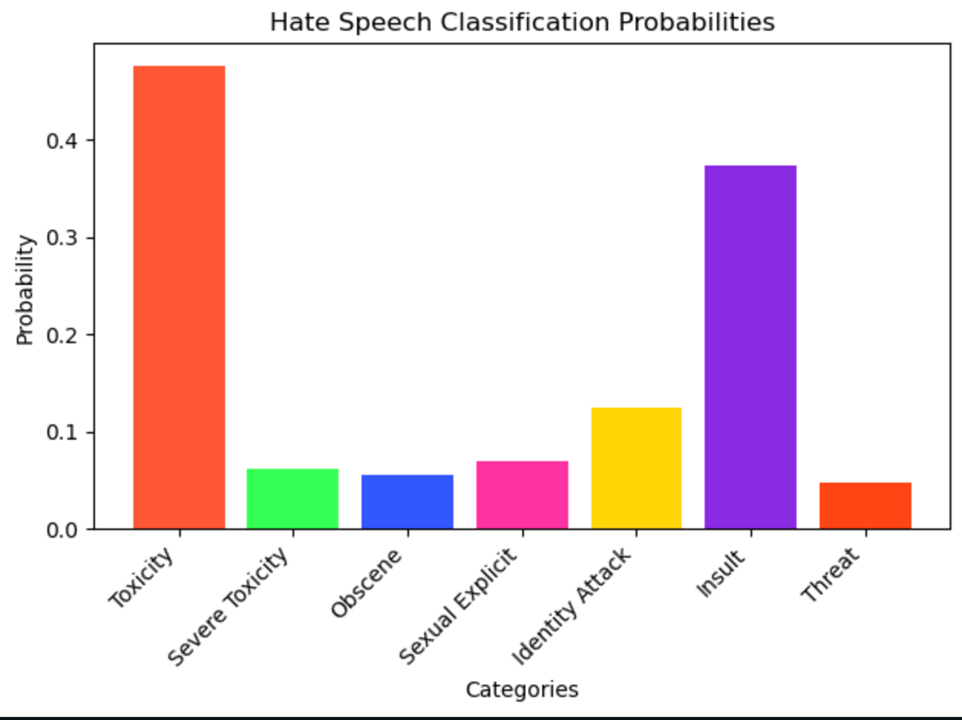
\includegraphics[scale=.6]{graficoIA}
    \SourceOrNote{Autoria Própria (2024)}
    \end{figure}